% ch6.tex
% This work is licensed under the Creative Commons Attribution-Noncommercial-Share Alike 3.0 New Zealand License.
% To view a copy of this license, visit http://creativecommons.org/licenses/by-nc-sa/3.0/nz
% or send a letter to Creative Commons, 171 Second Street, Suite 300, San Francisco, California, 94105, USA.


\chapter{Assim como reciclar$\ldots$}\label{ch:sortoflikerecycling}

Pense no montante de lixo que é criado todos os dias. Garrafas de água ou de refrigerante, pacotes de batata, embalagens de sanduíche, sacos de vegetais, carnes em bandejas de plástico, sacolas de compras de plástico, jornais, revistas e mais e mais$\ldots$
\par
Agora apenas imagine o que poderia acontecer se todo esse lixo fosse empilhado no entrada da sua garagem.

\begin{center}
\includegraphics*[width=100mm]{eps/trash.eps}
\end{center}

Claro que você reciclaria tudo que fosse possível. Que é uma coisa boa, pois ninguém gosta de andar por cima de uma montanha de lixo, a caminho da escola. Então, aquelas garrafas de vidro na lixeira de reciclagem serão derretidas e transformadas em novas garrafas e frascos; papel é transformado em papel reciclado; plástico se transforma em outras coisas de plástico --- então o gramado da frente da sua casa não desaparece em meio a uma pilha de lixo. Nós começamos a reutilizar alguns dos produtos que usamos, ao invés de tirar a mesma matéria prima da natureza de novo e de novo.

Reciclar ou reutilizar, no mundo da programação, é igualmente importante. Não porque o seu programa irá desaparecer debaixo de uma pilha de lixo --- mas se você não reutilizar algumas coisas que você faz, você eventualmente desgastará os seus dedos, digitando excessivamente.

Existem diversas maneiras de reutilizar código em Python (e nas linguagens de programação em geral), mas nós já vimos uma das maneiras, no Capítulo 3, com a função `range'. Funções\index{functions} são uma maneira de reutilizar código --- assim você pode escrever o código apenas uma vez, então usá-lo nos seus programas várias vezes. Vamos primeiro tentar um exemplo simples de função:

\begin{listing}
\begin{verbatim}
>>> def minhafuncao(nome):
...     print('Olá %s' % nome)
...
\end{verbatim}
\end{listing}

A função acima tem o nome `minhafuncao' e um parâmetro chamado `nome'. Um \emph{parâmetro} é uma variável que somente é acessível dentro do `corpo' da função (que é o bloco de código logo após a definição \code{def} (caso esteja se perguntando, \code{def} é uma abreviação para `defina'). Você pode executar a função, chamando-a pelo seu nome e os parâmetros entre parênteses:

\begin{listing}
\begin{verbatim}
>>> minhafuncao('Maria')
Olá Maria
\end{verbatim}
\end{listing}

\noindent
Nós podemos alterar a função para aceitar 2 parâmetros:

\begin{listing}
\begin{verbatim}
>>> def minhafuncao(nome, sobrenome):
...     print('Olá %s %s' % (nome, sobrenome))
...
\end{verbatim}
\end{listing}

\noindent
E então chamá-la da mesma maneira:

\begin{listing}
\begin{verbatim}
>>> minhafuncao('Maria', 'Almeida')
Olá Maria Almeida
\end{verbatim}
\end{listing}

\noindent
Ou nós poderíamos criar algumas variáveis e chamar a função com essas variáveis:

\begin{listing}
\begin{verbatim}
>>> nome = 'João'
>>> sobrenome = 'Roberto'
>>> minhafuncao(nome, sobrenome)
Olá João Roberto
\end{verbatim}
\end{listing}

\noindent
Nós podemos retornar valores de uma função, usando a expressão \code{return}\index{return}:

\begin{listing}
\begin{verbatim}
>>> def economias(trabalhos, entregas_jornal, gastos):
...     return trabalhos + entregas_jornal - gastos
...
>>> print(economias(10, 10, 5))
15
\end{verbatim}
\end{listing}

Esta função recebe 3 parâmetros, adiciona os dois primeiros (\code{trabalhos} e \code{entregas\_jornal}) antes de subtrair o último (\code{gastos}). O resultado é então retornado --- esse resultado pode ser usado como o valor de uma variável (da mesma forma que atribuímos valores à outras variáveis):

\begin{listing}
\begin{verbatim}
>>> minhas_economias = economias(20, 10, 5)
>>> print(minhas_economias)
25
\end{verbatim}
\end{listing}

\noindent
Porém, uma variável que nós usamos dentro do corpo de uma função, não será acessível (usável) após o fim da função:

\begin{listing}
\begin{verbatim}
>>> def teste_variavel():
...     a = 10
...     b = 20
...     return a * b
...
>>> print(teste_variavel())
200
>>> print(a)
Traceback (most recent call last):
  File "<stdin>", line 1, in <module>
NameError: name 'a' is not defined
\end{verbatim}
\end{listing} 

No exemplo acima, nós criamos uma função \code{teste\_variavel}, que multiplica o valor de duas variáveis (\code{a} e \code{b}) e retorna o resultado. Se nós chamarmos essa função usando o \code{print}, nós teremos o resultado: 200. Porém se nós tentarmos imprimir o valor de \code{a} (ou \code{b}, por exemplo), nós receberemos uma mensagem a erro ```a' is not defined'' (`a' não está definido). Isso é algo que chamamos de `\emph{escopo}'\index{scope}, no mundo da programação.
\par
Imagine uma função como uma pequena ilha flutuante no oceano --- e é muito longe para nadar da ilha até outro lugar qualquer. Ocasionalmente, um avião a sobrevoa e derruba pedaços de papel na ilha (são aqueles parâmetros, chegando na função) que os habitants então juntam e formam uma mensagem, colocam a mensagem dentro de uma garrafa e então lançam a garrafa ao mar (esse é o valor de retorno). O que os habitantes da ilha fazem, ou quantos deles foram necessários para formar a mensagem, não faz diferença à pessoa que pegou a garrafa e está lendo a mensagem. Essa é, provavelmente, a forma mais simples de explicar o escopo --- mas existe um pequeno problema nessa ideia. Um dos habitantes tem um par de binóculos gigante e pode ver tudo além do continente. Ele pode ver o que outras pessoas estão fazendo lá e isso pode afetar a mensagem que ele está criando:

\begin{listing}
\begin{verbatim}
>>> x = 100
>>> def teste2_variavel():
...     a = 10
...     b = 20
...     return a * b * x
... 
>>> print(teste2_variavel())
20000
\end{verbatim}
\end{listing}

Assim, mesmo que as variáveis \code{a} e \code{b} não possam ser usadas de fora da função, a variável \code{x} (que foi criada fora da função) pode ser usada dentro. Pense no habitante da ilha com o binóculos, espero que isso o ajude a entender melhor essa ideia.

\begin{center}
\includegraphics*[width=100mm]{eps/islanders.eps}
\end{center}

O laço `for' que nós criamos anteriormente para exibir as economias ao longo do ano, pode ser facilmente adicionado à uma função:

\begin{listing}
\begin{verbatim}
>>> def economias_no_ano(trabalhos, jornal, gastos):
...     economias = 0
...     for semana in range(1, 53):
...         economias = economias + trabalhos + jornal - gastos
...         print('Semana %s = %s' % (semana, economias))
...
\end{verbatim}
\end{listing}

Tente digitar essa função no terminal, e chamá-la com diferentes valores para \code{trabalhos}, \code{jornal}, e \code{gastos}:

\begin{listing}
\begin{verbatim}
>>> economias_no_ano(10, 10, 5)
Semana 1 = 15
Semana 2 = 30
Semana 3 = 45
Semana 4 = 60
Semana 5 = 75
Semana 6 = 90
Semana 7 = 105
Semana 8 = 120
Semana 9 = 135
Semana 10 = 150

(e por aí vai...)

>>> economias_no_ano(25, 15, 10)
Semana 1 = 30
Semana 2 = 60
Semana 3 = 90
Semana 4 = 120
Semana 5 = 150

(e por aí vai...)
\end{verbatim}
\end{listing}

Isso é um pouco mais eficiente que redigitar o laço `for' toda vez que você quiser tentar um valor diferente. Funções podem ser agrupadas no que chamamos de módulos, que tornam o Python muito mais eficiente.
\par
\noindent
\emph{Falaremos mais sobre módulos em breve.}

\section{Pedaços e peças}

Quando o Python é instalado no seu computador, uma montanha de funções e módulos também são instalados. Algumas funções são disponibilizadas por padrão. \code{range} é dessas funções, que nós já vimos. \code{file}\index{functions!file} é outra função que não usamos ainda.

\begin{WINDOWS}

Para ver como o \code{file} é usado, abra o Bloco de Notas, digite algumas palavras e então salve o arquivo como `teste.txt'.

\begin{enumerate}
 \item Clique no menu `Arquivo', então `Salvar',
 \item Clique duas vezes em `Meu Computador' na janela de Arquivo,
 \item Clique duas vezes em `Disco Local (C:)',
 \item No nome do arquivo (na parte debaixo) onde está `*.txt', coloque `teste.txt' 
\end{enumerate}

\begin{figure}
\begin{center}
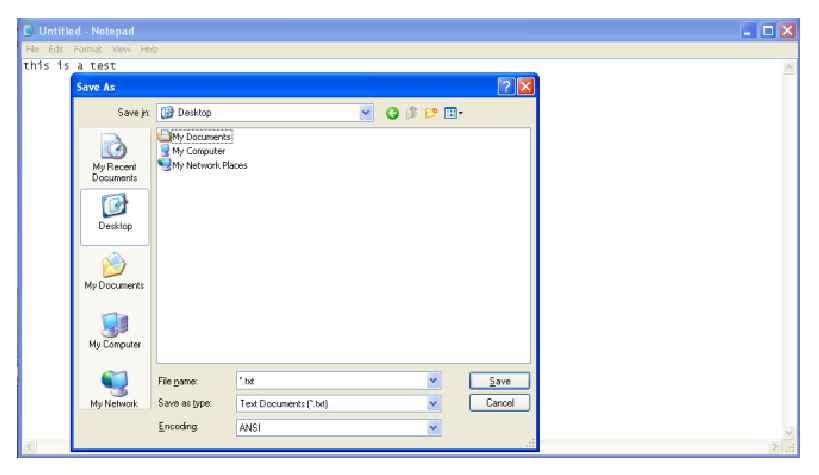
\includegraphics[width=65mm]{eps/figure17.eps}
\end{center}
\caption{Janela de Salvar Arquivo no Bloco de Notas.}\label{fig17}
\end{figure}

Abra o terminal do Python novamente e digite:

\begin{listing}
\begin{verbatim}
>>> f = open('c:\\teste.txt')
>>> print(f.read())
\end{verbatim}
\end{listing}

O conteúdo do arquivo que você acabou de criar será exibido.
\end{WINDOWS}

\begin{MAC}
Para ver como o \code{file} é usado, abra o Editor de Texto, clicando no ícone do editor (
\includegraphics[width=12mm]{eps/textedit-icon.eps}). Digite algumas palavras e então salve o arquivo na Mesa, clicando em Arquivo e Salvar, com o nome `teste.txt'.

\begin{figure}
\begin{center}
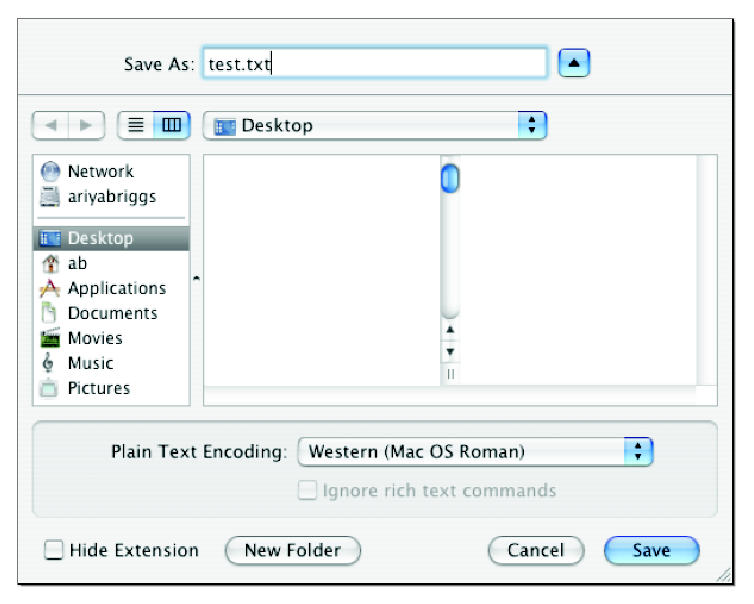
\includegraphics[width=65mm]{eps/figure18.eps}
\end{center}
\caption{Janela de Salvar Arquivo no Editor de Texto do Mac OS X.}\label{fig18}
\end{figure}

Abra o terminal do Python novamente e digite:

\begin{listing}
\begin{verbatim}
>>> f = open('Desktop/teste.txt')
>>> print(f.read())
\end{verbatim}
\end{listing}

O conteúdo do arquivo que você acabou de criar será exibido.
\end{MAC}

\begin{LINUX}
Para ver como o \code{file} é usado, abra um editor de texto, digite algumas palavras e então salve o arquivo no seu diretório `Home', clicando em Arquivo, Salvar e então selecionando o diretório `Home'. Digite o nome do arquivo `teste.txt` (veja na figura~\ref{fig19} por exemplo).

\begin{figure}
\begin{center}
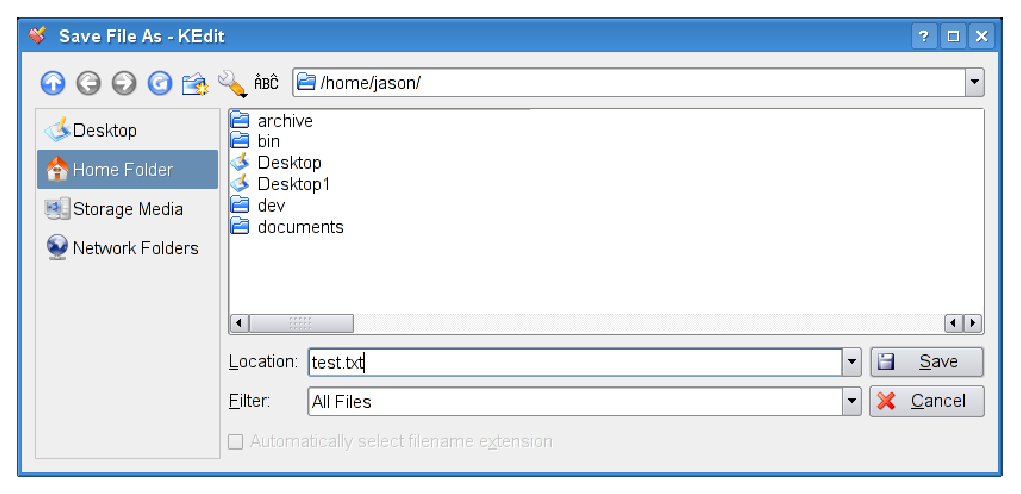
\includegraphics[width=65mm]{eps/figure19.eps}
\end{center}
\caption{Janela de Salvar Arquivo do Editor de Texto KEdit.}\label{fig19}
\end{figure}

Abra o terminal do Python novamente e digite:

\begin{listing}
\begin{verbatim}
>>> f = open('~/teste.txt')
>>> print(f.read())
\end{verbatim}
\end{listing}

\end{LINUX}

Então, o que esse pequeno trecho de código faz? A primeira linha chama a função \code{file}, passando o caminho do arquivo que você criou, como parâmetro. A função retorna um tipo de valor especial (chamado objeto) que representa um arquivo. Não é o arquivo em si; mas sim como se fosse um grande dedo apontando para o arquivo, dizendo ``AQUI ESTÁ ELE!!!'' O objeto de arquivo é armazenado na variável \code{f}.
\par
A próxima linha, chama uma função especial (\code{read}) no objeto de arquivo, para ler o seu conteúdo e imprimir o resultado no terminal. Por a variável \code{f} conter um objeto, isso significa que nós precisamos chamar a função `read' usando o símbolo ponto (.).

\fbox{\colorbox{PaleBlue}{\parbox{.75\linewidth} {
\par
O apêndice~\ref{app:builtinfunctions} (no final do livro) tem mais informações sobre as funções embutidas no Python.
\par
}}}

\section{Módulos}\index{modules}

Nós já vimos muitas formas diferentes de reutilizar códigos. Uma delas é criar uma função própria, ou então usar uma função pré-existente no Python (como o \code{range}, \code{file}, \code{int} e \code{str}). A outra é um tipo especial de função, em objetos --- que nós chamamos usando o símbolo ponto --- e a outra seria utilizando um módulo, que é uma forma de agrupar muitas funções e objetos, de forma eficiente. Um exemplo disso é o módulo `time'\index{modules!time}:

\begin{listing}
\begin{verbatim}
>>> import time
\end{verbatim}
\end{listing}

O comando `import' é usado para dizer ao Python que nós queremos usar um módulo. No exemplo acima, nós estamos dizendo que nós queremos usar o módulo `time'. Nós podemos então, chamar as funções e objetos disponíveis nesse módulo, usando o símbolo ponto, novamente:

\begin{listingignore}
\begin{verbatim}
>>> print(time.localtime())
(2006, 11, 10, 23, 49, 1, 4, 314, 1)
\end{verbatim}
\end{listingignore}

\code{localtime}\index{modules!time!localtime} é uma função \emph{dentro} do módulo `time', que retorna a data e hora atual, quebrada em partes individuais --- ano, mês, dia, hora, minuto, segundo, dia da semana, dia do ano e se é horário de verão ou não (1 se for, 0 se não). As partes individuais são armazenadas em uma tupla (veja \emph{Tuplas e Listas} na página~\pageref{tuplesandlists}. Você pode usar outra função do módulo `time' para converter a data e hora retornada pelo \code{localtime}, em algo mais legível:

\begin{listingignore}
\begin{verbatim}
>>> t = time.localtime()
>>> print(time.asctime(t))
Sat Nov 18 22:37:15 2006
\end{verbatim}
\end{listingignore}

\noindent
Nós podemos fazer tudo isso em apenas uma linha, se quisermos:

\begin{listingignore}
\begin{verbatim}
>>> print(time.asctime(time.localtime()))
Sat Nov 18 22:37:15 2006
\end{verbatim}
\end{listingignore}

Suponha que você queira perguntar a alguém um valor. Você pode fazer isso usando o comando \code{print} e o módulo `\code{sys}'\index{modules!sys} --- importando-o da mesma forma que fez com o módulo \code{time}:

\begin{listing}
\begin{verbatim}
import sys
\end{verbatim}
\end{listing}

Dentro do módulo `sys', tem um objeto chamado `stdin'\index{modules!sys!stdin} (abreviação de `standard input' ou `entrada padrão'). \code{stdin} tem um método (ou função) bastante útil, chamado \code{readline} --- que é usado para ler uma linha de texto que alguém digita (até que ela pressione Enter). Você pode testar o \code{readline}, usando os seguintes comandos no terminal do Python:

\begin{listing}
\begin{verbatim}
>>> print(sys.stdin.readline())
\end{verbatim}
\end{listing}

Se você digitar algumas palavras e pressionar a tecla Enter, o que você digitar será impresso no console. Relembre, por um momento, o código que escrevemos anteriormente, usando a expressão `if':

\begin{listing}
\begin{verbatim}
if idade >= 10 and idade <= 13:
    print('Você tem %s' % idade)
else:
    print('ahn?')
\end{verbatim}
\end{listing}

Ao invés de criar uma variável \code{idade} antecipadamente, nós podemos pedir à alguém para digitar o valor. Por que não, primeiramente, colocar o código em uma função$\ldots$

\begin{listing}
\begin{verbatim}
>>> def sua_idade(idade):
...     if idade >= 10 and idade <= 13:
...         print('Você tem %s' % idade)
...     else:
...         print('ahn?')
... 
\end{verbatim}
\end{listing}

Que pode ser chamada, passando um número como parâmetro. Primeiro, vamos testar para ver se funciona corretamente:

\begin{listing}
\begin{verbatim}
>>> sua_idade(9)
ahn?
>>> sua_idade(10)
Você tem 10
\end{verbatim}
\end{listing}

Agora que nós sabemos que não há problemas com a nossa função, podemos alterar ela para pedir a idade de uma pessoa:

\begin{listing}
\begin{verbatim}
>>> def sua_idade():
...     print('Por favor, insira a sua idade')
...     idade = int(sys.stdin.readline())
...     if idade >= 10 and idade <= 13:
...         print('Você tem %s' % idade)
...     else:
...         print('ahn?')
... 
\end{verbatim}
\end{listing}

Devido ao fato de que o \code{readline()} retorna o que uma pessoa digitou como um texto (em outras palavras, uma string), nós precisamos usar a função \code{int} para converter isso para um número (assim então, a expressão `if' funcionará corretamente --- veja \emph{Qual é a diferença} na página~\pageref{whatsthedifference} para mais informações a respeito sobre isso). Para tentar isso, chame a função \code{sua\_idade} sem nenhum parâmetro e então digite a sua idade quando o texto `Por favor, insira a sua idade' aparecer:

\begin{listingignore}
\begin{verbatim}
>>> sua_idade()
Por favor, insira a sua idade
10
Você tem 10
>>> sua_idade()
Por favor, insira a sua idade
15
ahn?
\end{verbatim}
\end{listingignore}

\noindent
\emph{A coisa mais importante em observar aqui, é que mesmo que você esteja digitando um número (no caso, 10 ou 15), a função `readline' sempre retornará uma string.}

\fbox{\colorbox{PaleBlue}{\parbox{.75\linewidth} {
O \code{sys} e \code{time} são apenas dois, de muitos módulos embutidos no Python. Para mais informações sobre alguns (não todos) módulos do Python, veja o Apêndice~\ref{app:afewpythonmodules}.
}}}

\section{Coisas para tentar}

\emph{Neste capítulo, nós vimos como fazer reciclagem em Python; através do uso de funções e módulos. Nós vimos um pouco sobre o escopo de uma variável, como variáveis de fora da função podem ser `vistas' de dentro, enquanto variáveis `de dentro' não podem ser acessadas de fora, e aprendemos como criar nossas próprias funções usando o \code{def}}

\subsection*{Exercício 1}
No exercício 2 do Capítulo~\ref{ch:againandagain}, nós criamos um laço `for' para descobrir quanto, de R\$100, nós ganhamos com juros, em um período de 10 anos. Esse laço `for' pode ser facilmente colocado em uma função. Tente criar uma função que recebe um valor inicial e uma taxa de juros. Você pode chamar a função usando o seguinte código:

\begin{listing}
\begin{verbatim}
calcular_juros(100, 0.03)
\end{verbatim}
\end{listing}

\subsection*{Exercício 2}
Pegue a função que você acabou de criar e faça ela calcular os juros em diferentes períodos --- como 5 anos ou 15 anos. Talvez você possa chamá-la usando o seguinte código:

\begin{listing}
\begin{verbatim}
calcular_juros(100, 0.03, 5)
\end{verbatim}
\end{listing}

\subsection*{Exercise 3}
Perhaps rather than a simple function, where we pass in the values as parameters, we can make a mini-program which asks someone for the values (using the \code{sys.stdin.readline()} function).  In this case, we'll call the function without any parameters at all:

\begin{listing}
\begin{verbatim}
calculate_interest()
\end{verbatim}
\end{listing}

\noindent
To create this mini-program requires a function that we haven't talked about yet: \code{float}. The \code{float} function is a bit like the \code{int} function, except it converts strings into what is called floating point numbers (which we discussed briefly in Chapter~\ref{ch:8multipliedby3.57}).  Floating point numbers are numbers with a decimal place (.), such as 20.3 or 2541.933.

\newpage
